\documentclass[a4paper,14pt]{extreport}

\usepackage{amsmath}
\usepackage{float}
\usepackage{graphicx}

\usepackage[utf8]{inputenc}
\usepackage[russian]{babel}

% поля:
\usepackage[left=2.5cm, right=2cm, top=2cm, bottom=2cm]{geometry}
\linespread{1}
\usepackage{indentfirst} % отделять первую строку раздела абзацным отступом
\setlength\parindent{5ex}
\addto{\captionsrussian}{\renewcommand*{\contentsname}{Содержание}}
\usepackage[hidelinks]{hyperref} % гиперссылки в содержании
\usepackage{graphicx}
\usepackage{float}
\usepackage{amsmath}
\renewcommand*{\thesection}{\arabic{section}}


\begin{document}
	
	\begin{titlepage}
		\begin{center}
			\large
			МИНИСТЕРСТВО ОБРАЗОВАНИЯ И НАУКИ\\ РОССИЙСКОЙ ФЕДЕРАЦИИ
			
			\textbf{Федеральное агентство по образованию}
			\vspace{0.5cm}
			
			УНИВЕРСИТЕТ ИТМО
			\vspace{0.25cm}
			
			Факультет компьютерных технологий и управления
			
			Кафедра систем управления и информатики
			\vfill
			
			
			Студент: Артемов Кирилл\\
			группа P4135\\
					
			\textsc{Лабораторная работа №2}\\[5mm]
			
			{\LARGE Решение обратной задачи кинематики}
			\bigskip
			
		\end{center}
		\vfill
		
		\newlength{\ML}
		\settowidth{\ML}{«\underline{\hspace{0.7cm}}» \underline{\hspace{2cm}}}
		\hfill\begin{minipage}{0.4\textwidth}
			Преподаватель\\
			\underline{\hspace{\ML}} А.\,А.~Пыркин\\
			«\underline{\hspace{0.7cm}}» \underline{\hspace{2cm}} 2016 г.
		\end{minipage}%
		\bigskip

		\vfill
		
		\begin{center}
			Санкт-Петербург, 2016 г.
		\end{center}
	\end{titlepage}
	
	\pagenumbering{gobble}
	\section{Цель работы}
	Решение обратной задачи кинематики (ОЗК).
	
	\section{Исходные данные}
	Шестизвенный манипулятор с вращательными звеньями.
	\begin{table}[H]
		\caption{\label{tab:canonsummary}Параметры DH.}
		\begin{center}
			\begin{tabular}{|c|c|c|c|c|}
				\hline
				Link & $a_i$ & $\alpha_i $ & $d_i$ & $\theta_i$ \\
				\hline
				$1$ & $0$ & $\frac{\pi}{2}$ & $d_1$ & $0$ \\
				\hline
				$2$ & $a_2$ & $0$ & $0$ & $0$ \\
				\hline
				$3$ & $0$ & $\frac{\pi}{2}$ & $0$ & $\frac{\pi}{2}$ \\
				\hline
				$4$ & $0$ & $-\frac{\pi}{2}$ & $d_4$ & $0$ \\
				\hline
				$5$ & $0$ & $\frac{\pi}{2}$ & $0$ & $0$ \\
				\hline
				$6$ & $0$ & $0$ & $d_6$ & $0$ \\
				\hline
			\end{tabular}
		\end{center}
	\end{table} 
	Дана матрица однородных преобразований (4x4).
	\begin{equation}
		H^0_6 = 
		\begin{pmatrix}
			R & o\\
			0 & 1
		\end{pmatrix}
	\end{equation}
	где вектор положения схвата:
	\begin{equation}
		o^0_6 = 
		\begin{pmatrix}
			o_x\\
			o_y\\
			o_z
		\end{pmatrix}
	\end{equation}
	матрица ориентации схвата:
	\begin{equation}
		R^0_6 = 
		\begin{pmatrix}
			r_{11} & r_{12} & r_{13}\\
			r_{21} & r_{22} & r_{23}\\
			r_{31} & r_{32} & r_{33}\\
		\end{pmatrix}
	\end{equation}
	
	\section{Ход выполнения работы}
	Так как оси вращения $z_4, z_5, z_6$ пересекаются в точке $o_c$, то задача разделяется на две подзадачи:
	\begin{enumerate}
		\item ОЗК по положению - нахождение $q_1, q_2, q_3$
		\item ОЗК по ориентации - нахождение $q_4, q_5, q_6$	
	\end{enumerate}

	\subsection{ОЗК по положению}
	\begin{figure}[H]
		\center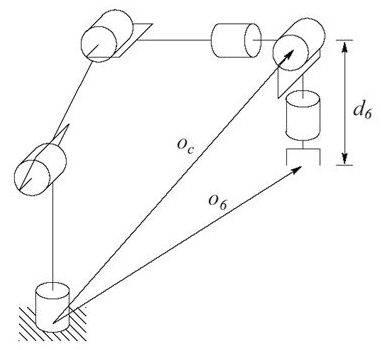
\includegraphics[width=0.3\linewidth]{decoupling.png}
		\caption{Kinematic decoupling}
		\label{fig:scr1}
	\end{figure}
	Для начала следует найти вектор $o^0_c$:
	\begin{equation}
		o^0_c = o^0_6 - d_6R^0_6 
		\begin{bmatrix}
			0\\
			0\\
			1
		\end{bmatrix}
	\end{equation}
	Далее, получив уравнения для проекции каждой из координат точки $o_c$ на соответстующие оси, преступим к геометрическому нахождению углов $q_1, q_2, q_3$.
	\begin{equation}
		\begin{bmatrix}
			x_c\\
			y_c\\
			z_c			
		\end{bmatrix}
		=		
		\begin{bmatrix}
			o_x - d_6r_{13}\\		
			o_y - d_6r_{23}\\
			o_z - d_6r_{33}						
		\end{bmatrix}
	\end{equation}
	
	\subsubsection{Решение для $q_1$}
	\begin{figure}[H]
		\center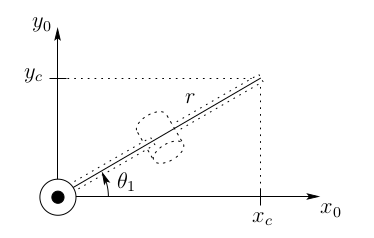
\includegraphics[width=0.3\linewidth]{position_q1.png}
		\caption{Угол $q_1 = \theta_1$}
		\label{fig:scr2}
	\end{figure}
	\begin{center}
		$q_1^1 = atan2(y_c, x_c)$\\
		$q_1^2 = \pi  + atan2(y_c, x_c)$\\
		где $x_c \neq 0, y_c \neq 0$	
	\end{center}	
	
	\subsubsection{Решение для $q_3$}
	\begin{figure}[H]
		\center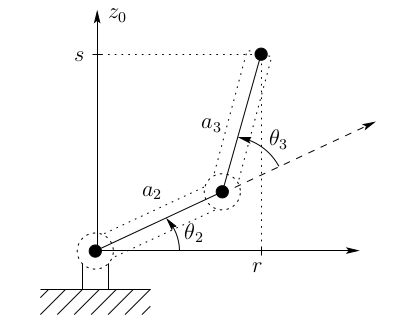
\includegraphics[width=0.3\linewidth]{position_q3.png}
		\caption{Угол $q_3 = \theta_3$}
		\label{fig:scr3}
	\end{figure}
	По теореме синусов получим:
	\begin{center}
		$s^2 + r^2 = a_2^2 + a_3^2 - 2a_2a_3 \cos{(\pi - q_3)}$\\
		$\cos q_3 = \frac{s^2 + r^2 - a^2_2 - a^2_3}{2a_2a_3} = D$\\
		$s = z_c - d_1$\\
		$r = \sqrt{x_c^2 + y_c^2}$\\
		$q_3^1 = atan2( \sqrt{1 - D^2}, D)$
		$q_3^2 = atan2(-\sqrt{1 - D^2}, D)$
	\end{center}
	
	
	\subsubsection{Решение для $q_2$}
	
	Тут, необходимо заметить, что плоская часть манипулятора в одну и ту же точку может прийти четырьмя разными способами. Т.е для каждого из $q_1$ имеем два $q_3$ и четыре $q_2$. Таким образом получаем четыре конфигурации манипулятора для углов $q_1, q_2, q_3$.
	
	\begin{center}
		$q_2^{1,2} = atan2(s, r) - atan2(a_3 \sin q_3, a_2 + a_3 \cos q_3)$
		$q_2^{3,4} = pi - atan2(s, r) - atan2(a_3 \sin q_3, a_2 + a_3 \cos q_3)$
	\end{center}
	
	 
	
	
	\subsection{ОЗК по ориентации}
	Положение схвата описывается следующим выражением:
	\begin{equation}
		R^0_6 = R^0_3 R^3_6
	\end{equation}
	Выразим матрицу поворота $R^3_6$ через известную $R^0_3$ и заданную $R^0_6$:
	\begin{equation}
		R^3_6 = (R^0_3)^{-1} R^0_6 = (R^0_3)^T R^0_6 = 
		\begin{bmatrix}
		h_{11} & h_{12} & h_{13}\\
		h_{21} & h_{22} & h_{23}\\
		h_{31} & h_{32} & h_{33}\\
		\end{bmatrix}
	\end{equation}
	Запишем соотношение заданной матрицы и матрицы $R_6^3$:
	\begin{equation}
		\begin{bmatrix}
			h_{11} & h_{12} & h_{13}\\
			h_{21} & h_{22} & h_{23}\\
			h_{31} & h_{32} & h_{33}\\
		\end{bmatrix}		
		=
		\begin{bmatrix}
			c_{q_1}c_{q_2}c_{q_3} & -c_{q_1}s_{q_2}s_{q_3} & s_{q_1}\\
			s_{q_1}c_{q_2}c_{q_3} & -s_{q_1}s_{q2}s_{q_3} & -c_{q_1}\\
			s_{q_2}s_{q_3}	& c_{q_2}c_{q_3} & 0
		\end{bmatrix}
		\begin{bmatrix}
			r_{11} & r_{12} & r_{13}\\
			r_{21} & r_{22} & r_{23}\\
			r_{31} & r_{32} & r_{33}\\
		\end{bmatrix}		
	\end{equation}	
	Найдем матрицу $ZYZ-Euler Angle Transformation$
	\begin{equation}
		R_{ZYZ} =
		\begin{bmatrix}
			c_{\phi} c_{\theta} c_{\psi} - s_{\phi} s_{\psi} & -c_{\phi} c_{\theta} s_{\psi} - s_{\phi} s_{\psi} & c_{\phi}s_{\theta} \\
			s_{\phi} c_{\theta} c_{\psi} - c_{\phi} s_{\psi} & c_{\phi} c_{\psi} - s_{\phi} c_{\theta} s_{\psi} & s_{\phi}s_{\theta} \\
			-s_{\theta} c_{\psi} & s_{\theta} s_{\psi} & c_{\theta}
		\end{bmatrix}
	\end{equation}	
	Пусть:
	\begin{equation}
		\begin{bmatrix}
			q_4\\
			q_5\\
			q_6
		\end{bmatrix}
		=
		\begin{bmatrix}
			\phi\\
			\theta\\
			\psi
		\end{bmatrix}
	\end{equation}	
	Теперь приравням $R^3_6 = R_{ZYZ}$, получим девять уравнений, решая совместно которые найдем нужные нам углы.
	
	\subsubsection{Решение для $\theta \neq \pi k$} 
	Если $h_{13} \neq h_{23}$, то $\sin{\theta} \neq 0$, следовательно $\cos{\theta} = h_{33}\neq \pm 1, \sin{\theta} = \pm \sqrt{1 - h_{33}^2}$.
	\begin{equation}
		\theta_1,2 = atan2(\pm \sqrt{1 - h_{33}^2}, h_{33})\\
	\end{equation}		
	Если $\sqrt{1 - h_{33}^2} > 0$, тогда:
	\begin{center}
		$\phi_1 = atan2(h_{23}, h_{13})$\\
		$\psi_1 = atan2(h_{32}, -h_{31})$
	\end{center}
	Если $\sqrt{1 - h_{33}^2} < 0$, тогда:
	\begin{center}
		$\phi_2 = atan2(-h_{23}, -h_{13})$\\
		$\psi_2 = atan2(-h_{32}, h_{31})$
	\end{center}

	\subsubsection{Решение для $\theta = \pi k$}
	Если $h_{13} = h_{23} = 0$ и $h_{31} = h_{32} = 0$, то $h_{33} = \pm 1 = \cos \theta$.
	Если $h_{33} > 0$, то $\cos{\theta} = 1, \sin{\theta} = 0$, следовательно $\theta = 0$
	\begin{center}
		$\phi + \psi = atan2(h_{21}, h_{11}) = atan2(-h_{12}, h_{11})$
	\end{center}
	Если $h_{33} < 0$, то $\cos{\theta} = -1, \sin \theta = 0$, следовательно $\theta = \pi$
	\begin{center}
		$\phi - \psi = atan2(h_{21},h_{11}) = atan2(-h_{12}, -h_{11})$
	\end{center}
	В обоих последних случаях углы $\phi$ и $\psi$ могут быть любыми, т.е. существует бесконечное количество решений полученных уравнений.
	
	\section{Моделирование}
	
	Для проверки полчуенных решений мною была написана программа на языке программирования Pyton, результаты работы которой представленны ниже.
	
	Для приведенных примеров $q_1 = 0$. 
	
	На рисунках буквой а) отмечена заданная конфигурация манипулятора для котороый была решена прямая задача кинематики и получена матрица $H^0_6$. Буквой б) -- четыре возможные конфигурации манипулятора для заданной точки $oc$ (Конфигурации 2 и 4 изображены зеркально, для большей наглядности).
	Розовой точке соответствует положение схвата манипулятора. Красная точка изображает положение точки $oc$, найденной ранее в разделе 3.1.  
	
	\begin{figure}[H]
		\begin{minipage}[h]{0.4\linewidth}
			\center{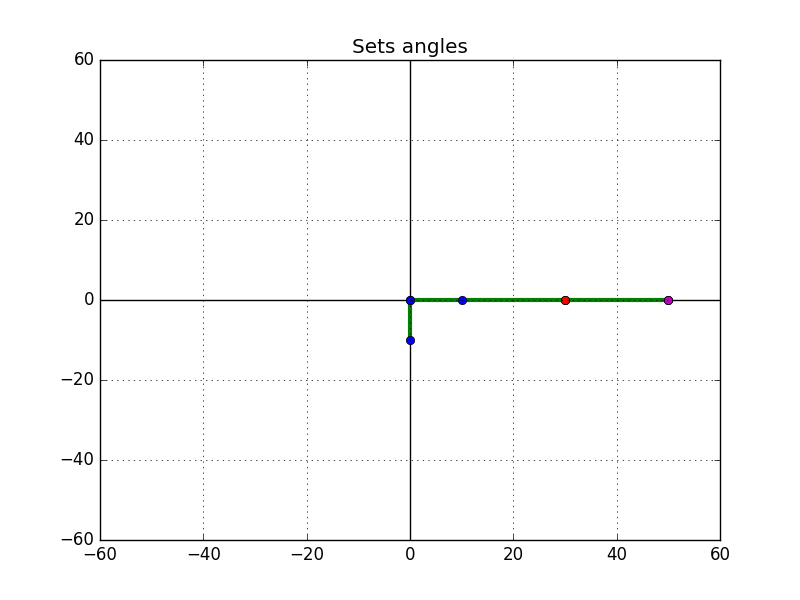
\includegraphics[width=1.2\linewidth]{sets_1.png} \\ а)}
		\end{minipage}
		\hfill
		\begin{minipage}[h]{0.4\linewidth}
			\center{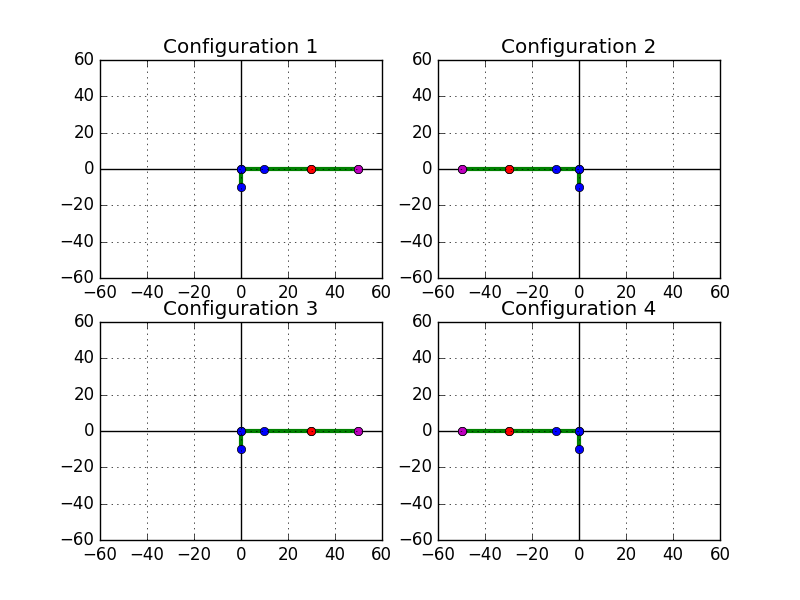
\includegraphics[width=1.2\linewidth]{res_1.png} \\ б)}
		\end{minipage}
		\caption{Для заданных углов в градусах $[0, 0, 0, 0, 0, 0]$.}
		\label{ris:image1}
	\end{figure}

	\begin{figure}[H]
		\begin{minipage}[h]{0.4\linewidth}
			\center{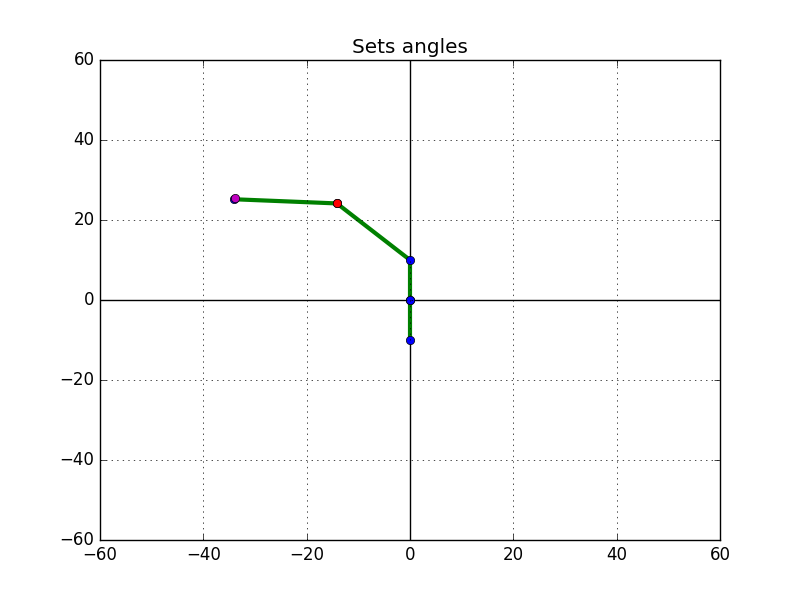
\includegraphics[width=1.2\linewidth]{sets_2.png} \\ а)}
		\end{minipage}
		\hfill
		\begin{minipage}[h]{0.4\linewidth}
			\center{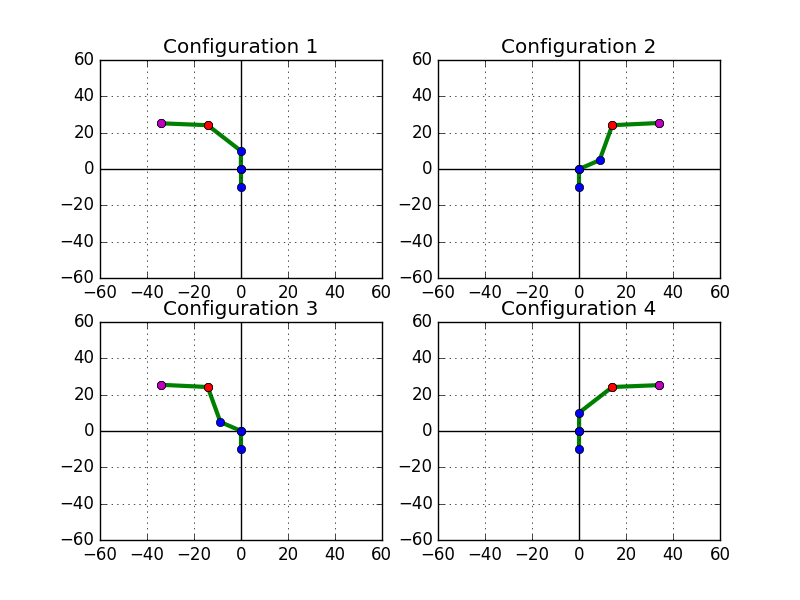
\includegraphics[width=1.2\linewidth]{res_2.png} \\ б)}
		\end{minipage}
		\caption{Для заданных углов в градусах $[0, 90, 45, 13, 42, 201]$.}
		\label{ris:image2}
	\end{figure}
	
	И последнее, что остается проверить это ориентацию схвата. Для этого решим прямую задачу кинематики для полученных значений обобщенных координат и сравним их.
	\begin{equation}
		R_{init}
		\begin{bmatrix}
			-0.04587165 & -0.15718776 & -0.98650281 & -33.87219189\\
			0.63195955 &  0.76024362 & -0.15052164 & -3.01043271\\
			0.77364263 & -0.63033455 &  0.06446268 & 35.43138918\\
			0. & 0. & 0. & 1. \\
		\end{bmatrix}		
	\end{equation}	
	\begin{equation}
		R_{result}
		\begin{bmatrix}
		-0.04587831 & -0.15718265 & -0.98650332& -33.87220197\\
		0.63196448 &  0.76023956 & -0.15052147 & -3.01042941\\
		0.77363821 & -0.63034073 &  0.06445535 & 35.43124262\\
		0.         &  0.         &  0.        &   1.        
		\end{bmatrix}		
	\end{equation}	
	Матрицы равны с точностью до трех знаков.
	
	\section{Вывод}
	
	Итак, проделав долгий и тяжелый путь от нахождения параметров Денавита-Хартенберга, решения прямой задачи кинематики, обратной по положению и ориентации, моделировании и анализе полученных результатов можно с уверенностью сказать -- задача выполнена. 
	
\end{document}